\subsection{Architektūros įtaka}
\label{subsec:rez_architektura}

Lyginamos trys konvoliucinių blokų konfigūracijos kiekvienai užduočiai (žr.~\ref{tab:rez_architektura} lentelę). Validavimo metrikų kitimas per epochas pateiktas \ref{fig:rez_architektura_image} ir~\ref{fig:rez_architektura_keystroke} pav.

\begin{table}[H]
    \centering
    \caption{Architektūros tyrimo rezultatai. Geriausi variantai paryškinti.}
    \begin{tabular}{|l|l|c|c|c|}
        \hline
        Užduotis & Variantas & \texttt{val\_acc} & \texttt{val\_loss} & \texttt{test\_acc} \\
        \hline
        \multirow{3}{*}{Vaizdai}
            & Small \texttt{(16, 32)}        & $0{,}8254$ & $0{,}4955$ & $0{,}8305$ \\ \cline{2-5}
            & \textbf{Medium \texttt{(32, 64, 128)}} & $\mathbf{0{,}8413}$ & $\mathbf{0{,}8387}$ & $0{,}8178$ \\ \cline{2-5}
            & \textbf{Large \texttt{(64, 128, 256)}} & $0{,}8201$ & $0{,}4792$ & $\mathbf{0{,}8432}$ \\
        \hline
        \multirow{3}{*}{Laiko eilutės}
            & Small \texttt{(32,)}           & $0{,}6792$ & $1{,}5507$ & $0{,}7467$ \\ \cline{2-5}
            & \textbf{Medium \texttt{(64, 128)}} & $\mathbf{0{,}6917}$ & $\mathbf{1{,}0635}$ & $0{,}7200$ \\ \cline{2-5}
            & Large \texttt{(64, 128, 256)}  & $0{,}6042$ & $1{,}4302$ & $0{,}6233$ \\
        \hline
    \end{tabular}
    \label{tab:rez_architektura}
\end{table}


\begin{figure}[H]
    \centering
    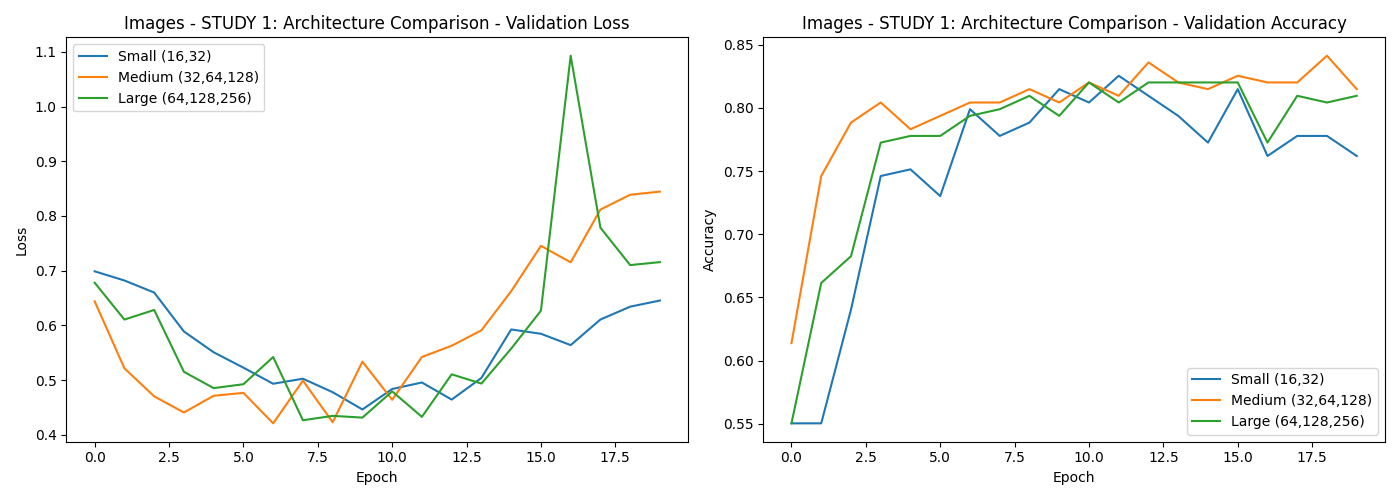
\includegraphics[width=0.9\linewidth]{3Lab/results/architecture/img_comparison.png}
    \caption{Architektūros tyrimas – vaizdų užduotis}
    \label{fig:rez_architektura_image}
\end{figure}

\begin{figure}[H]
    \centering
    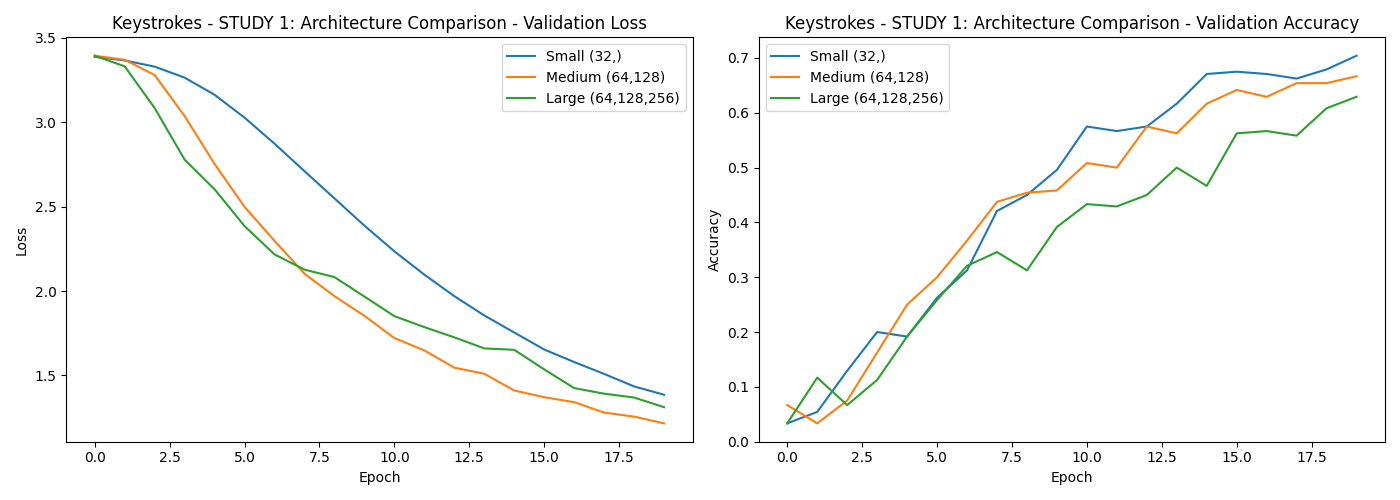
\includegraphics[width=0.9\linewidth]{3Lab/results/architecture/ks_comparison.png}
    \caption{Architektūros tyrimas – laiko eilučių užduotis}
    \label{fig:rez_architektura_keystroke}
\end{figure}

Pastebimi rezultatai:
\begin{itemize}
    \item Vaizdams \textbf{vidutinė architektūra} \texttt{(32, 64, 128)} pasiekė didžiausią validavimo tikslumą ($0{,}8413$), tačiau didžiausias \texttt{test\_acc} ($0{,}8432$) buvo gautas su \textbf{didele} \texttt{(64, 128, 256)} architektūra – tai rodo, kad gilesnis tinklas geriau generalizuoja, nors validavimo aibėje šiek tiek labiau persimokė.
    \item Laiko eilutėms didžiausią validavimo tikslumą gavo \texttt{(64, 128)} architektūra ($0{,}6917$). Dvigubinant filtrų skaičių iki \texttt{(64, 128, 256)} tinklas pradeda sparčiai persimokyti – $1\,500$ įrašų aibei tai per gilus modelis.
\end{itemize}
